% Source: graduate-coursework/Sp26/CSCE775/course_notes/ch5_exercises/exercise_5_1.tex
% Description: Three backup diagrams. (a) The DP diagram for $v_\pi$ fans out over all actions and all next states but only goes one step deep. (b) The MC diagram for $v_\pi$ follows a single sampled trajectory from a \textit{state

\documentclass[border=4pt]{standalone}
\usepackage{amsmath, amssymb}
\usepackage{graphicx}
\usepackage{tikz}
\usepackage{xcolor}
\usetikzlibrary{positioning}

\definecolor{garnet}{HTML}{73000A}
\definecolor{black90}{HTML}{363636}
\definecolor{atlantic}{HTML}{466A9F}

\begin{document}
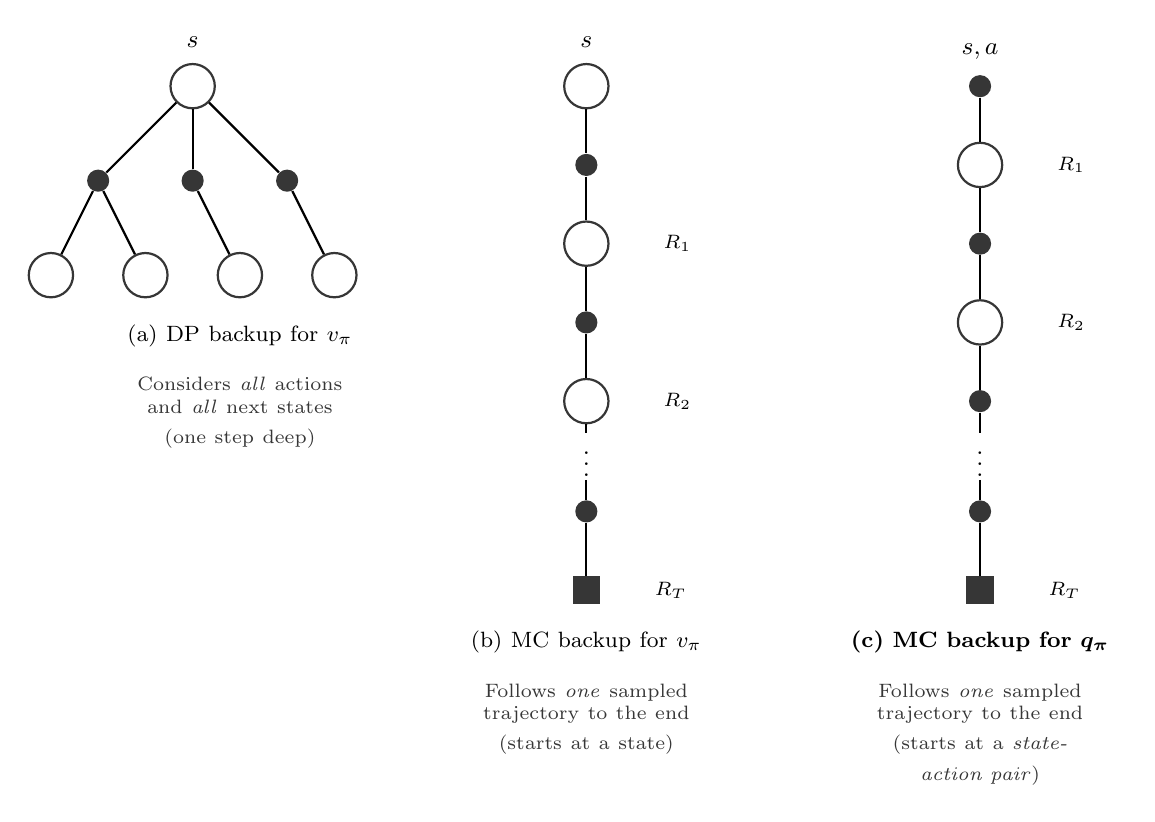
\begin{tikzpicture}[
    state/.style={circle, draw=black90, thick, minimum size=16pt, inner sep=0pt},
    action/.style={circle, fill=black90, minimum size=8pt, inner sep=0pt},
    terminal/.style={rectangle, fill=black90, minimum size=10pt, inner sep=0pt},
    every node/.style={font=\small},
    level distance=18mm,
    sibling distance=14mm
]

% ── Diagram A: DP backup for v_π ──
\begin{scope}[shift={(-5,0)}]
    \node[state] (s) at (0,0) {};
    \node[above=2pt of s] {$s$};

    \node[action] (a1) at (-1.2,-1.2) {};
    \node[action] (a2) at (0,-1.2) {};
    \node[action] (a3) at (1.2,-1.2) {};

    \node[state] (s1) at (-1.8,-2.4) {};
    \node[state] (s2) at (-0.6,-2.4) {};
    \node[state] (s3) at (0.6,-2.4) {};
    \node[state] (s4) at (1.8,-2.4) {};

    \draw[thick] (s) -- (a1);
    \draw[thick] (s) -- (a2);
    \draw[thick] (s) -- (a3);
    \draw[thick] (a1) -- (s1);
    \draw[thick] (a1) -- (s2);
    \draw[thick] (a2) -- (s3);
    \draw[thick] (a3) -- (s4);

    \node[below=6pt of s3, text width=3.5cm, align=center] (alabel) {\footnotesize (a) DP backup for $v_\pi$};
    \node[below=4pt of alabel, text width=3.5cm, align=center, text=black90] {\scriptsize Considers \textit{all} actions \\ and \textit{all} next states \\ (one step deep)};
\end{scope}

% ── Diagram B: MC backup for v_π ──
\begin{scope}[shift={(0,0)}]
    \node[state] (ms) at (0,0) {};
    \node[above=2pt of ms] {$s$};

    \node[action] (ma1) at (0,-1.0) {};
    \node[state] (ms1) at (0,-2.0) {};
    \node[action] (ma2) at (0,-3.0) {};
    \node[state] (ms2) at (0,-4.0) {};

    % dots
    \node at (0,-4.7) {$\vdots$};

    \node[action] (ma3) at (0,-5.4) {};
    \node[terminal] (mt) at (0,-6.4) {};

    \draw[thick] (ms) -- (ma1);
    \draw[thick] (ma1) -- (ms1);
    \draw[thick] (ms1) -- (ma2);
    \draw[thick] (ma2) -- (ms2);
    \draw[thick] (ms2) -- (0,-4.4);
    \draw[thick] (0,-5.0) -- (ma3);
    \draw[thick] (ma3) -- (mt);

    \node[right=16pt of ms1] {\scriptsize $R_1$};
    \node[right=16pt of ms2] {\scriptsize $R_2$};
    \node[right=16pt of mt] {\scriptsize $R_T$};

    \node[below=6pt of mt, text width=3.5cm, align=center] (blabel) {\footnotesize (b) MC backup for $v_\pi$};
    \node[below=4pt of blabel, text width=3.5cm, align=center, text=black90] {\scriptsize Follows \textit{one} sampled \\ trajectory to the end \\ (starts at a state)};
\end{scope}

% ── Diagram C: MC backup for q_π (THE ANSWER) ──
\begin{scope}[shift={(5,0)}]
    \node[action] (qa) at (0,0) {};
    \node[above=2pt of qa] {$s, a$};

    \node[state] (qs1) at (0,-1.0) {};
    \node[action] (qa1) at (0,-2.0) {};
    \node[state] (qs2) at (0,-3.0) {};
    \node[action] (qa2) at (0,-4.0) {};

    % dots
    \node at (0,-4.7) {$\vdots$};

    \node[action] (qa3) at (0,-5.4) {};
    \node[terminal] (qt) at (0,-6.4) {};

    \draw[thick] (qa) -- (qs1);
    \draw[thick] (qs1) -- (qa1);
    \draw[thick] (qa1) -- (qs2);
    \draw[thick] (qs2) -- (qa2);
    \draw[thick] (qa2) -- (0,-4.4);
    \draw[thick] (0,-5.0) -- (qa3);
    \draw[thick] (qa3) -- (qt);

    \node[right=16pt of qs1] {\scriptsize $R_1$};
    \node[right=16pt of qs2] {\scriptsize $R_2$};
    \node[right=16pt of qt] {\scriptsize $R_T$};

    \node[below=6pt of qt, text width=3.5cm, align=center] (qlabel) {\footnotesize \textbf{(c) MC backup for} $\boldsymbol{q_\pi}$};
    \node[below=4pt of qlabel, text width=3.5cm, align=center, text=black90] {\scriptsize Follows \textit{one} sampled \\ trajectory to the end \\ (starts at a \textit{state-action pair})};
\end{scope}

\end{tikzpicture}
\end{document}
